\documentclass{article}

\usepackage{graphicx}
\usepackage{tikz}
\usepackage{tikzsymbols}
\usetikzlibrary{calc,patterns,shapes.geometric}
\pagestyle{empty}
\usepackage[margin=0pt]{geometry}
\geometry{papersize={14in,12in}}

\def\centerarc[#1](#2)(#3:#4:#5){\draw[#1] ($(#2)+({#5*cos(#3)},{#5*sin(#3)})$) arc (#3:#4:#5);}

\begin{document}
	\begin{figure}
		\centering
		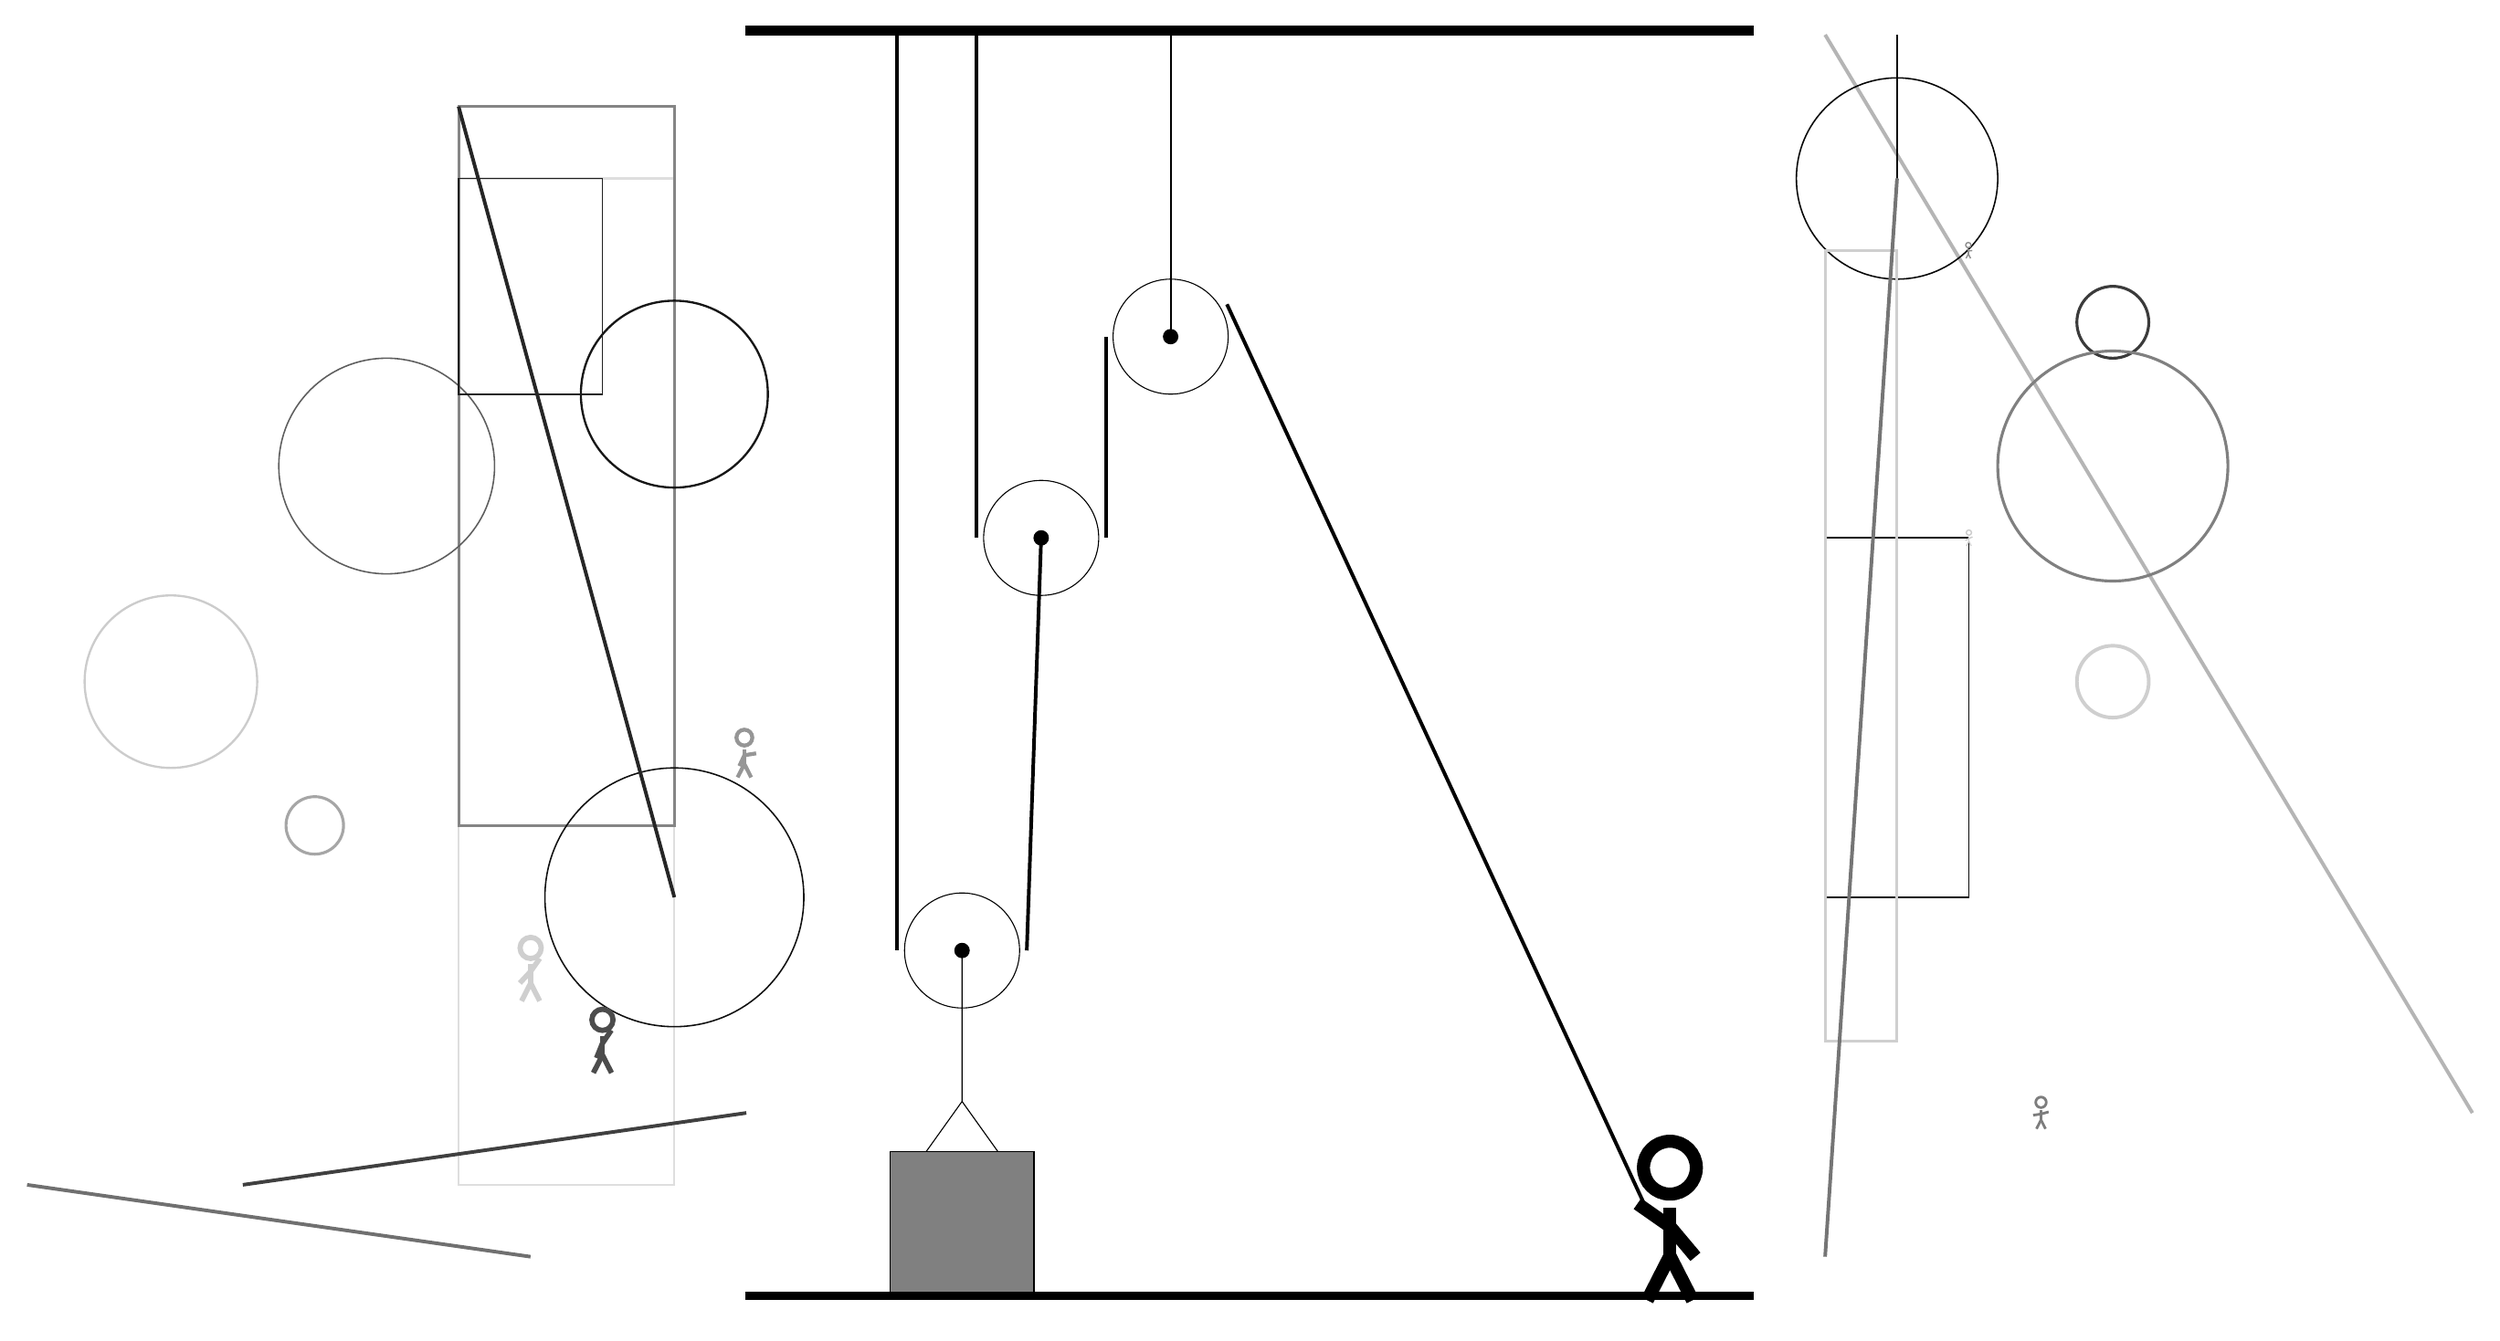
\begin{tikzpicture}
			%%%%% START %%%%%
			
			\draw[fill=black] (-2, 14) rectangle (12, 14.125);
			
			\draw (1, 1.26) circle (0.8);
			\draw[fill=black] (1, 1.26) circle (0.1);
			
			\draw (2.1, 7.0) circle (0.8);
			\draw[fill=black] (2.1, 7.0) circle (0.1);
			
			\draw (3.9, 9.8) circle (0.8);
			\draw[fill=black] (3.9, 9.8) circle (0.1);
			\draw[thick] (3.9, 9.8) -- (3.9, 14);
			
			\draw (1, 1.26) -- (1, -0.84) -- (0.5, -1.54) -- (1.5, -1.54) -- (1, -0.84);
			\draw[fill=black!50] (0, -1.54) rectangle (2, -3.54);
			
			\draw[line width=0.5mm] (0.1, 14) -- (0.1, 1.26);
			\centerarc[line width=0.5mm](1, 1.26)(180:360:0.9);
			\draw[line width=0.5mm](1.9, 1.26) -- (2.1, 7.0);
			\draw[line width=0.5mm] (1.2, 14) -- (1.2, 7.0);
			\centerarc[line width=0.5mm](2.1, 7.0)(180:360:0.9);
			\draw[line width=0.5mm](3.0, 7.0) -- (3.0, 9.8);
			\centerarc[line width=0.5mm](3.9, 9.8)(30:180:0.9);
			\draw[line width=0.5mm] (4.683, 10.25) -- (10.5, -2.3);
			
			\draw[line width=0.3mm, color=black!13] (-3, 12) rectangle (-6, -2);
			
			\draw[line width=0.4mm, color=black!48] (-3, 13) rectangle (-6, 3);
			\draw[line width=0.5mm, color=black!75](-2, -1) -- (-9, -2);
			\draw[line width=0.5mm, color=black!29](13, 14) -- (22, -1);
			\draw [line width=0.5mm, color=black!19](17, 5) circle (0.5);
			
			\draw[line width=0.2mm, color=black!96] (13, 7) rectangle (15, 2);
			
			\draw[line width=0.3mm, color=black!97] (14, 12) rectangle (14, 14);
			
			\draw [line width=0.4mm, color=black!77](17, 10) circle (0.5);
			\draw [line width=0.3mm, color=black!91](-3, 9) circle (1.3);
			\draw [line width=0.2mm, color=black!98](14, 12) circle (1.4);
			\node[line width=0.6mm, color=black!41] at (-2, 4) {\Strichmaxerl[3][65][9]};
			\draw [line width=0.4mm, color=black!35](-8, 3) circle (0.4);
			\node[line width=0.2mm, color=black!20] at (15, 7) {\Strichmaxerl[1][28][23]};
			
			\node[line width=0.4mm, color=black!51] at (16, -1) {\Strichmaxerl[2][8][16]};
			\draw[line width=0.5mm, color=black!56](-5, -3) -- (-12, -2);
			\draw [line width=0.2mm, color=black!63](-7, 8) circle (1.5);
			
			\node[line width=0.4mm, color=black!19] at (-5, 1) {\Strichmaxerl[4][47][55]};
			\draw [line width=0.2mm, color=black!94](-3, 2) circle (1.8);
			\draw[line width=0.4mm, color=black!19] (13, 0) rectangle (14, 11);
			\draw[line width=0.2mm, color=black!88] (-4, 12) rectangle (-6, 9);
			\draw[line width=0.5mm, color=black!85](-6, 13) -- (-3, 2);
			
			\draw [line width=0.3mm, color=black!20](-10, 5) circle (1.2);
			
			\draw [line width=0.4mm, color=black!50](17, 8) circle (1.6);
			\node[line width=0.3mm, color=black!70] at (-4, 0) {\Strichmaxerl[4][68][56]};
			\draw[line width=0.5mm, color=black!54](14, 12) -- (13, -3);
			\node[line width=0.5mm, color=black!44] at (15, 11) {\Strichmaxerl[1][89][6]};
			
			\node at (10.8, -2.5) {\Strichmaxerl[10][-35][-50]};
			
			\draw[fill=black] (-2, -3.5) rectangle (12, -3.6);
			
			%%%%% END %%%%%
		\end{tikzpicture}
	\end{figure}	
\end{document}